\documentclass{beamer}

\usepackage[cm-default]{fontspec}
\usepackage{xunicode}
\usepackage{xltxtra}
\setmainfont[Mapping=tex-text]{DejaVu Sans}

\usepackage{graphicx}
\usepackage{amssymb}

\usetheme{Pittsburgh}
\useinnertheme{rounded}
\usefonttheme{serif}
\usecolortheme{beaver}

\title[Αναδρομικές Συναρτήσεις στο λ-λογισμό]
      {Αναπαράσταση Αναδρομικών Συναρτήσεων στο λ-λογισμό}
\author{Σταύρος Αρώνης, Ειρήνη Αρβανίτη}
\date{14 Σεπτεμβρίου 2010}
\institute{Εφαρμογές της λογικής στην Πληροφορική\\Σχολή ΗΜΜΥ, ΕΜΠ}

\setbeamertemplate{navigation symbols}{}
\setbeamertemplate{footline}{
  \leavevmode
  \hbox{
    \begin{beamercolorbox}[wd=.5\paperwidth,ht=2.5ex,dp=1.125ex,right]
      {author in head/foot}
      \usebeamerfont{title in head/foot}
      \insertshortauthor
      \hspace{.3cm}
    \end{beamercolorbox}%
    
    \begin{beamercolorbox}[wd=.40\paperwidth,ht=2.5ex,dp=1.125ex,left]
      {title in head/foot}
      \usebeamerfont{author in head/foot}\
      \hspace{.3cm}
      \insertshorttitle
    \end{beamercolorbox}
    
    \begin{beamercolorbox}[wd=.10\paperwidth,ht=2.5ex,dp=1.125ex,center]
      {title in head/foot}
      \usebeamerfont{author in head/foot}
      \insertframenumber/\inserttotalframenumber
    \end{beamercolorbox}
  }
  \vskip0pt
}

\AtBeginSection[]
{
  \begin{frame}<beamer>
    \frametitle{Επισκόπηση}
    \tableofcontents[currentsection, hideothersubsections]
  \end{frame}
}

\begin{document}

\begin{frame}
  \titlepage
  \begin{center}
    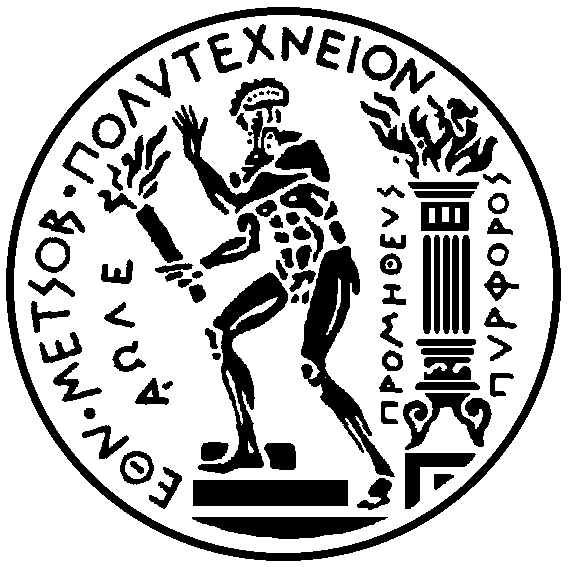
\includegraphics[height=2cm]{pyrforos.png}
  \end{center}
\end{frame}

\section*{Επισκόπηση}

\begin{frame}
  \tableofcontents[hidesubsections]
\end{frame}

\section{Πρωταρχικά αναδρομικές συναρτήσεις}

\subsection{Ορισμός}

\begin{frame}
  \frametitle{Ορισμός}
  \begin{itemize}
  \item Οι \textbf{πρωταρχικά αναδρομικές συναρτήσεις} είναι
    συναρτήσεις με πεδίο ορισμού το $\mathbb{N}^k$ και σύνολο τιμών το
    $\mathbb{N}$.\pause
  \item Η κλάση τους είναι η μικρότερη που περιέχει τις ακόλουθες
    θεμελιώδεις συναρτήσεις και είναι κλειστή ως προς τα ακόλουθα
    σχήματα κλεισίματος (επαγωγικό σύνολο).
  \end{itemize}
\end{frame}

\subsection{Θεμελιώδεις συναρτήσεις}

\begin{frame}
  \frametitle{Θεμελιώδεις συναρτήσεις}
  \begin{itemize}
  \item Η σταθερή συνάρτηση με τιμή 0: $$Z_0=0$$
  \item Η συνάρτηση που παίρνει έναν αριθμό και επιστρέφει τον
    επόμενο: $$S_1(n)=n+1$$
  \item Οι συναρτήσεις
    προβολής: $$U^i_n(x_1,\ldots,x_i,\ldots,x_n)=x_i$$
  \end{itemize}
\end{frame}

\subsection{Σχήματα κλεισίματος}

\subsubsection{Σύνθεση}

\begin{frame}
  \frametitle{Σύνθεση}
  \begin{itemize}
  \item Αν έχουμε τις πρωταρχικά αναδρομικές συναρτήσεις: $$H_m, G1_n,
    \ldots, GM_n$$
  \item Τότε και η
    $$
    F_n(x_1,\ldots,x_n) =
    H_m(G1_n(x_1,\ldots,x_n),\ldots,GM_n(x_1,\ldots,x_n))
    $$
    είναι πρωταρχικά αναδρομική.
  \end{itemize}
\end{frame}

\subsubsection{Πρωταρχική Αναδρομή}

\begin{frame}
  \frametitle{Πρωταρχική Αναδρομή}
  \begin{itemize}
  \item Αν έχουμε τις πρωταρχικά αναδρομικές συναρτήσεις:
    $$
    G_n, H_{n+2}
    $$
  \item Τότε και η
    $$
    \left\{
    \begin{array}{llr@{}l}
      F_{n+1}(x_1,\ldots,x_n, 0)     &=&    G_n(&x_1,\ldots,x_n) \\
      F_{n+1}(x_1,\ldots,x_n, S_1(y))&=&H_{n+2}(&x_1,\ldots,x_n, y ,\\
      & &        &F_n(x_1,\ldots,x_n, y))
    \end{array}
    \right.
    $$
    είναι πρωταρχικά αναδρομική.
  \end{itemize}
\end{frame}

\subsection{Παραδείγματα πρωταρχικά αναδρομικών συναρτήσεων}

\begin{frame}
  \frametitle{Παραδείγματα πρωταρχικά αναδρομικών συναρτήσεων}
  \begin{itemize}
  \item Η συνάρτηση προηγούμενος:
    $$
    \left\{
    \begin{array}{ll}
      P_1(0)      &= Z_0\\
      P_1(S_1(x)) &= U^1_2(x,P(x))
    \end{array}
    \right.
    $$
    \pause
  \item Η συνάρτηση πρόσθεσης:
    $$
    \left\{
    \begin{array}{ll}
      Add_2(x, 0)      &= U^1_1(x)\\
      Add_2(x, S_1(y)) &= S_1(U^3_3(x, y , Add_2(x, y)))
    \end{array}
    \right.
    $$
    ή πιο απλά:
    $$
    \left\{
    \begin{array}{ll}
      Add_2(x, 0)      &= x\\
      Add_2(x, S_1(y)) &= S_1(Add_2(x, y))
    \end{array}
    \right.
    $$
    \pause
  \item Η συνάρτηση αφαίρεσης:
    $$
    \left\{
    \begin{array}{ll}
      Sub_2(x, 0)      &= x\\
      Sub_2(x, S_1(y)) &= P_1(Sub_2(x, y))
    \end{array}
    \right.
    $$
  \end{itemize}
\end{frame}

\begin{frame}
  \frametitle{Παραδείγματα πρωταρχικά αναδρομικών συναρτήσεων}
  \begin{itemize}
  \item Η συνάρτηση πολλαπλασιασμού:
    $$
    \left\{
    \begin{array}{ll}
      Mult_2(x, 0)      &= Z_0\\
      Mult_2(x, S_1(y)) &= Add_2(x, Mult_2(x, y))
    \end{array}
    \right.
    $$
    \pause
  \item Η συνάρτηση << ίσο με 0 >>:
    $$
    \left\{
    \begin{array}{ll}
      EZ(0)      &= S_1(Z_0)\\
      EZ(S_1(x)) &= Z_0
    \end{array}
    \right.
    $$
  \end{itemize}
\end{frame}

\subsection{Απαρίθμηση πρωταρχικά αναδρομικών συναρτήσεων}

\begin{frame}
  \frametitle{Απαρίθμηση πρωταρχικά αναδρομικών συναρτήσεων}
  \begin{itemize}
  \item Οι πρωταρχικά αναδρομικές συναρτήσεις είναι αριθμήσιμο
    σύνολο. \pause
  \item Για την απαρίθμηση μπορούμε να χρησιμοποιήσουμε π.χ. το
    ακόλουθο σχήμα βασισμένο στα αριθμητικά του G\"odel
    \footnote{\htmladdnormallink{\tiny
        http://en.wikipedia.org/wiki/G\"odel\_number}
      {http://en.wikipedia.org/wiki/G\%C3\%B6del_number}}:
    \begin{itemize}
    \item Οι θεμελιώδεις συναρτήσεις:
      $$
      \begin{array}{l}
        Z_0 \rightarrow 1 \\
        S_1 \rightarrow 2*3^1 \\
        U^i_n \rightarrow 2^2*3^n*5^i
      \end{array}
      $$
    \end{itemize}
  \end{itemize}
\end{frame}

\begin{frame}
  \frametitle{Απαρίθμηση πρωταρχικά αναδρομικών συναρτήσεων}
  \begin{itemize}
  \item Το σχήμα σύνθεσης:
    \begin{itemize}
    \item Αν έχουμε την αντιστοίχιση:
      $$
      \begin{array}{l}
        H_m \rightarrow N_H,\\
        G1_n \rightarrow N_{G1},\\
        \ldots,\\
        GM_n \rightarrow N_{GM}
      \end{array}
      $$
    \item Τότε η $F_n(x_1,\ldots,x_n) =
      H_m(G1_n(x_1,\ldots,x_n),\ldots,GM_n(x_1,\ldots,x_n))$
      αντιστοιχεί στο:
      $$2^3*3^n*5^{N_H}*7^{N_{G1}}*\ldots*Prime_{m+3}^{N_{GM_n}}$$
    \end{itemize}                   
  \end{itemize}
\end{frame}

\begin{frame}
  \frametitle{Απαρίθμηση πρωταρχικά αναδρομικών συναρτήσεων}
  \begin{itemize}
  \item Το σχήμα πρωταρχικής αναδρομής:
    \begin{itemize}
    \item Αν έχουμε την αντιστοίχιση:
      $$
      \begin{array}{l}
        G_n \rightarrow N_Γ,\\
        H_{n+2} \rightarrow N_H
      \end{array}
      $$
    \item Τότε η 
      $$
      \left\{
      \begin{array}{llr@{}l}
        F_{n+1}(x_1,\ldots,x_n, 0)     &=&    G_n(&x_1,\ldots,x_n) \\
        F_{n+1}(x_1,\ldots,x_n, S_1(y))&=&H_{n+2}(&x_1,\ldots,x_n, y ,\\
        & &        &F_n(x_1,\ldots,x_n, y))
      \end{array}
      \right.
      $$
      αντιστοιχεί στο:
      $$ 2^4*3^n*5^{N_G}*7^{N_H} $$
    \end{itemize}                   
  \end{itemize}
\end{frame}

\begin{frame}
  \frametitle{Απαρίθμηση πρωταρχικά αναδρομικών συναρτήσεων}
  \begin{itemize}
  \item Η απαρίθμηση δεν αντιστοιχεί σε κάθε ακέραιο μια έγκυρη
    πρωταρχικά αναδρομική συνάρτηση αλλά είναι εφικτό να ελεγχθεί αν
    ένας ακέραιος αντιστοιχεί σε έγκυρη συνάρτηση: \pause
    \begin{itemize}
    \item Παραγοντοποιούμε τον αριθμό
    \item Ελέγχουμε τη δύναμη του 2 για να δούμε αν είναι απλή
      περίπτωση
    \item Αν είναι σχήμα κλεισίματος, ελέγχουμε αναδρομικά κάθε μια
      συνάρτηση που περιλαμβάνεται όπως και το ίδιο το σχήμα
      κλεισίματος.
    \end{itemize}
    \pause
  \item Είναι επίσης εύκολο να βρούμε πόσα ορίσματα εχει μια συνάρτηση
    που αντιστοιχεί σε έναν κωδικό
  \item $Legal(x)=0|1$ και $Args(x)=n$
  \end{itemize}
\end{frame}

\section{Αναδρομικές συναρτήσεις}

\subsection{Γιατί δεν αρκεί η πρωταρχική αναδρομή}

\begin{frame}
  \frametitle{Γιατί δεν αρκεί η πρωταρχική αναδρομή}
  \begin{itemize}
  \item Δεν είναι όλες οι << υπολογίσιμες >> συναρτήσεις
    πρωταρχικά αναδρομικές!
    \pause
  \item Έστω η συνάρτηση $f(x)$ με τύπο:
    $$
    f(x)=\left\{
    \begin{array}{ll}
      0           &, Legal(x) \neq 1 \vee Args(x) \neq 1\\
      FX_1(x) + 1 &, $διαφορετικά$
    \end{array}
    \right.
    $$
    όπου $FX_1$ η συνάρτηση με κωδικό $x$.
  \item Υπολογίσιμη συνάρτηση.
  \end{itemize}
\end{frame}

\begin{frame}
  \frametitle{Γιατί δεν αρκεί η πρωταρχική αναδρομή}
  \begin{itemize}
  \item Έστω ότι η $f$ είναι πρωταρχικά αναδρομική.\pause
  \item Τότε έχει κάποιον κωδικό έστω $N_f$.\pause
  \item Άρα $f(N_f) = FN_f(N_f) + 1 = f(N_f) + 1$.\pause
  \item Άτοπο!
  \end{itemize}
\end{frame}

\begin{frame}
  \frametitle{Γιατί δεν αρκεί η πρωταρχική αναδρομή}
  \begin{itemize}
  \item Η συνάρτηση Ackermann:
    $$
    \left\{
    \begin{array}{ll}
      A(0,n) &= n+1\\
      A(m,0) &= A(m-1,1)\\
      A(m,n) &= A(m-1, A(m,n-1))
    \end{array}
    \right.
    $$
  \item Υπολογίσιμη.
  \item Δεν μπορεί να γραφεί με πρωταρχική αναδρομή 
    \footnote{
      \htmladdnormallink{\tiny
        http://home.manhattan.edu/~gregory.taylor/thcomp/pdf-files/ackerman.pdf}
                        {http://home.manhattan.edu/~gregory.taylor/thcomp/pdf-files/ackerman.pdf}}.
  \end{itemize}
\end{frame}

\subsection{Αναδρομικές συναρτήσεις}

\begin{frame}
  \frametitle{Αναδρομικές συναρτήσεις}
  \begin{itemize}
  \item Μερικές συναρτήσεις.
    $$F_n(a_1,\ldots,a_n)=
    \left\{
    \begin{array}{l}
      b\\
      \bot
    \end{array}
    \right.
    $$
  \item Περιλαμβάνουν:
    \begin{itemize}
    \item Θεμελιώδεις συναρτήσεις.
    \item Σχήματα κλεισίματος:
      \begin{itemize}
      \item Σύνθεση
      \item Πρωταρχική αναδρομή
      \item \textbf{Ελαχιστοποίηση}
      \end{itemize}
    \end{itemize}
  \end{itemize}
\end{frame}

\subsection{Σχήμα ελαχιστοποίησης}

\begin{frame}
  \frametitle{Σχήμα ελαχιστοποίησης}
  \begin{itemize}
  \item Αν έχουμε την αναδρομική συνάρτηση $F_{n+1}(y,x_1,\ldots,x_n)$
  \item Τότε και η:
    $$
    \begin{array}{l}
      G_n = \mu y(F_{n+1}(y,x_1,\ldots,x_n)) = z \Leftrightarrow \\ \\
      \left\{
      \begin{array}{l}
	\exists y_0,\ldots,y_n $ τέτοια ώστε $ \\
    	y_i = F_{n+1}(i, x_1,\ldots, x_n), $ για $ i=0,1,\ldots,z \\
    	y_i > 0, $ για $ i=0,1,\ldots,z-1 \\
    	y_z = 0
      \end{array}
      \right.
    \end{array}
    $$
    είναι αναδρομική.
  \end{itemize}
\end{frame}

\subsection{Αοριστία}

\begin{frame}
  \frametitle{Αοριστία}
  Η χρήση του παραπάνω σχήματος εισάγει αοριστίες:
  \begin{itemize}
  \item Αν $y_i = F_{n+1}(i, x_1,\ldots, x_n)$ δεν είναι ποτέ ίσο με
    $0$.
  \item Αν $y_i > 0$ για $i=0,1,\ldots,w-1$ και $y_w$ δεν ορίζεται.
  \end{itemize}
\end{frame}

\section{Στοιχεία λ-λογισμού}

\subsection{Συντακτικό}

\begin{frame}
  \frametitle{Συντακτικό}
  \begin{itemize}
  \item Ένας λ-όρος μπορεί να είναι μια μεταβλητή.$$x$$
  \item Αν $t$ είναι λ-όρος και $x$ είναι μεταβλητή, τότε $$\lambda
    x.t$$ είναι επίσης λ-όρος.
  \item Αν $t, u$ είναι λ-όροι, τότε $$(t)u$$ είναι επίσης λ-όρος.
  \end{itemize}
\end{frame}

\subsection{Αντικατάσταση}

\begin{frame}
  \frametitle{Αντικατάσταση}
  
  Αν $t$, $M$ είναι λ-όροι και $x$ είναι μεταβλητή, τότε η
  αντικατάσταση της $x$ από τον $t$ στον όρο $M$, συμβολίζεται με
  $M[x:=t]$
  \begin{itemize}
  \item $x[x:=t] \equiv t$
  \item $y[x:=t] \equiv y$
  \item $((P)Q)[x:=t] \equiv (P[x:=t])Q[x:=t]$
  \item $(\lambda y . P)[x:=t] \equiv \lambda y . (P[x:=t])$
  \item $(\lambda x . P)[x:=t] \equiv \lambda x . P$
  \end{itemize}
\end{frame}

\subsection{β-συστολή}

\begin{frame}
  \frametitle{β-συστολή}
  $\rightarrow _\beta$ είναι η μικρότερη διμελής σχέση στο $\Lambda$
  ώστε να ισχύει ότι $$(\lambda x . P)Q \rightarrow _\beta P[x:=Q]$$
  και είναι κλειστή για τους ακόλουθους κανόνες:
  \begin{itemize}
  \item $P \rightarrow _\beta P^{\prime} \Rightarrow \forall x \in V
    : \lambda x . P \rightarrow _\beta \lambda x .  P^{\prime}$
  \item $P \rightarrow _\beta P^{\prime} \Rightarrow \forall Z \in
    \Lambda : (P)Z \rightarrow _\beta (P^{\prime})Z$
  \item $P \rightarrow _\beta P^{\prime} \Rightarrow \forall Z \in
    \Lambda : (Z)P \rightarrow _\beta (Z)P^{\prime}$
  \end{itemize} \pause
  	\[ \]
  	´Ενας όρος $M$ είναι μία \textit{$\beta$ - κανονική μορφή} εάν
    δεν υπάρχει όρος $N$ ώστε $M \rightarrow _\beta N$.
\end{frame}

\subsection{β-αναγωγή}

\begin{frame}
  \frametitle{β-αναγωγή}
  Η σχέση $\twoheadrightarrow _\beta$ είναι η μεταβατική και αυτοπαθής
  κλειστότητα της σχέσης $\rightarrow _\beta$
  \begin{itemize}
  \item $P \rightarrow _{\beta} P ^{\prime} \Rightarrow P
    \twoheadrightarrow _{\beta} P ^{\prime}$
  \item $P \twoheadrightarrow _{\beta} P ^{\prime} \cap P ^{\prime}
    \twoheadrightarrow _{\beta} P ^{\prime \prime} \Rightarrow P
    \twoheadrightarrow _{\beta} P ^{\prime \prime}$
  \item $P \twoheadrightarrow _{\beta} P$
  \end{itemize} \pause
  Ισχύει η ακόλουθη πρόταση:
  $$
  \small
  \begin{array}{ll}
    M \twoheadrightarrow _\beta N \Leftrightarrow 
    & $Είτε $ M \equiv N $ είτε υπάρχουν $ M_1, M_2,\ldots M_n $ ώστε $ \\
    & M \equiv M_1 $ και N $ \equiv M_n $ και για κάθε $ i (1 \leq i \leq n-1),\\
    & M_i \rightarrow _\beta M_{i+1}
  \end{array}
  $$
\end{frame}

\subsection{β-ισοδυναμία}

\begin{frame}
  \frametitle{β-ισοδυναμία} 
  Η σχέση $ =_\beta$ είναι η μεταβατική, αυτοπαθής και συμμετρική
  κλειστότητα της σχέσης $\rightarrow _\beta$
  \begin{itemize}
  \item $P \rightarrow  _\beta P^\prime \Rightarrow P  =_\beta P^\prime $
  \item $P =_\beta P^\prime \cap P^\prime =_\beta P ^{\prime \prime}
    \Rightarrow P =_\beta P ^{\prime \prime}$
  \item $P =_\beta P$
  \item $P  =_\beta P^\prime \Rightarrow P^\prime =_\beta P$
  \end{itemize} \pause
  Ισχύει η ακόλουθη πρόταση:
  $$
  \small
  \begin{array}{ll}
    M =_\beta N \Leftrightarrow 
    & $ Υπάρχουν $ M_1, M_2,\ldots M_n $ με $ M \equiv M_1 $ και $ N
    \equiv M_n \\
    & $ και για κάθε i $ (1 \leq i \leq n-1) $ έχουμε $ M_i
    \twoheadrightarrow _\beta M_{i+1}\\
    & $ ή $ M_{i+1} \twoheadrightarrow _\beta M_i
  \end{array}
  $$
\end{frame}

\begin{frame}
  \frametitle{Κανονικοποίηση}
  \begin{itemize}
  \item \textbf{Θεώρημα Church-Rosser:} Αν $t \twoheadrightarrow
    _\beta u, v$ τότε μπορεί να βρεθεί $w$ τέτοιο ώστε $ u, v
    \twoheadrightarrow _\beta w$.
    \begin{figure}
      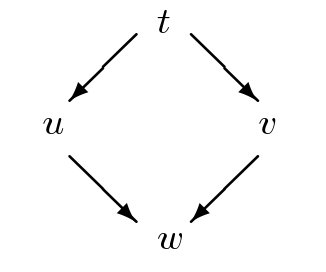
\includegraphics[scale=0.3]{CR.jpg} 
    \end{figure} \pause
  \item \textbf{Ορισμός}: Έστω $t \twoheadrightarrow _\beta u$ και $u$
    είναι $\beta$-κανονική μορφή. Τότε ο όρος $u$ λέγεται
    $\beta$-κανονική μορφή του $t$.
  \item \textbf{Πόρισμα}: Ένας όρος $t$ έχει το πολύ μια κανονική
    μορφή.
  \end{itemize}
\end{frame}

\begin{frame}
  \frametitle{Κανονικοποίηση}
  \textbf{Πόρισμα}: $u =_\beta v \Leftrightarrow$ Υπάρχει όρος $t$
  ώστε $u, v \twoheadrightarrow _\beta t$.
  \begin{itemize}
  \item $(\Leftarrow)$ Προφανές από τον ορισμό της $\beta$-ισοδυναμίας.
  \item $(\Rightarrow)$ Aν κάποιος μπορεί να συμπεράνει ότι $u =_\beta v$,
    τότε είναι εύκολο να παρατηρήσει ότι υπάρχουν όροι $u = t_0,
    t_1,\ldots, t_{2n-1}, t_{2n} = v$. Εφαρμόζοντας επανειλημμένα το
    θεώρημα Church-Rosser, καταλήγουμε σε έναν όρο $w$ τέτοιον ώστε
    $u, v \twoheadrightarrow _\beta w$.
    \begin{figure} [!ht]
      \centering
      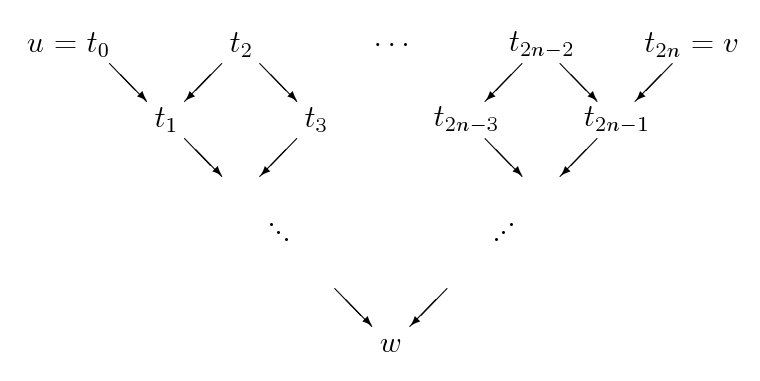
\includegraphics[scale=0.3] {CR1.jpg}
    \end{figure}
  \end{itemize}
\end{frame}

\begin{frame}
  \frametitle{Κανονικοποίηση}
  \begin{itemize}
  \item Δεν έχουν όλοι οι όροι κανονικές μορφές, π.χ. ο όρος $\Omega
    \equiv (\lambda x . xx) \lambda x . xx$. Αν όμως υπάρχει, τότε
    είναι μοναδική.
  \item Ένας όρος ο οποίος έχει κανονική μορφή ονομάζεται
    κανονικοποιήσιμος. Αυτό δε συνεπάγεται ότι οποιαδήποτε αναγωγή
    οδηγεί στην κανονική μορφή του.
  \item Κάθε όρος που έχει άπειρη αναγωγή περιέχει τον όρο
    $\Omega$. Ωστόσο, το αντίστροφο δεν ισχύει.
  \item Ένας όρος που δεν έχει καμία άπειρη αναγωγή ονομάζεται ισχυρά
    κανονικοποιήσιμος.
  \end{itemize}
\end{frame}

\begin{frame}
  \frametitle{Αριστερότερη Αναγωγή}
  \begin{itemize}
  \item \textbf{Αριστερότερο redex} ενός μη κανονικού όρου $t$ είναι
    το redex στο οποίο το "$(\lambda$" βρίσκεται αριστερότερα από κάθε
    άλλο "$(\lambda$" του $t$.
  \item \textbf{Αριστερότερη αναγωγή} καλείται μία ακολουθία $t_0,
    t_1, \ldots, t_n, \ldots$ τέτοια ώστε $\forall n: t_n \rightarrow
    _\beta t_{n+1}$ με συστολή του αριστερότερου redex στον
    $t_n$.
  \item \textbf{Συμβολισμός:} $t \rightarrow _l t^\prime$ , $t
    \twoheadrightarrow _l t^\prime$
  \item Για δεδομένα $t$, $n$ η αριστερότερη αναγωγή είναι
    μοναδική. Αν $t$ κανονικοποιήσιμος τότε η αριστερότερη αναγωγή
    καταλήγει στην κανονική μορφή του $t$.
  \end{itemize}
\end{frame}

\begin{frame}
  \frametitle{Αναγωγή κεφαλής}
  \begin{itemize}
  \item \textbf{Πρόταση:} Κάθε $\lambda$-όρος $t$ γράφεται μοναδικά με
    μία από τις ακόλουθες μορφές:
    $$(1): \lambda x_1 \ldots \lambda x_n . (x) t_1 \ldots t_m$$ 
    $$(2): \lambda x_1 \ldots \lambda x_n . ((\lambda x . u) v) t_1
    \ldots t_m$$ \pause
  \item \textbf{Απόδειξη:} Με επαγωγή στον όρο $t$.
  \item $t$ μεταβλητή: (1) όπου $n=m=0$ \pause
  \item $t = \lambda x . t^\prime$: Από Ε.Υ. $t^\prime$ γράφεται
    κατάλληλα, συνεπώς το ίδιο και ο $t$ \pause
  \item $t = (t^\prime) t^{\prime \prime}$:
    \begin{itemize}
    \item $t^\prime$ $\lambda$-αφαίρεση: (2) όπου $n=m=0$ \pause
    \item αν $t^\prime$ δεν είναι $\lambda$-αφαίρεση, τότε $t^\prime =
      (w) w_1 \ldots w_k$, όπου $w$ μεταβλητή ή redex, άρα $t = ((w)
      w_1 \ldots w_k) t^{\prime \prime}$, δηλαδή (1) ή (2) όπου $n=0$
    \end{itemize}
  \end{itemize}
\end{frame}

\begin{frame}
  \frametitle{Αναγωγή κεφαλής}
  \begin{itemize}
  \item Κάθε όρος $t = \lambda x_1 \ldots \lambda x_n . (x) t_1 \ldots
    t_m$ ονομάζεται κανονική μορφή κεφαλής.\pause
  \item Επιπλέον, αν $t = \lambda x_1 \ldots \lambda x_n . ((\lambda x
    . u) v) t_1 \ldots t_m$, τότε $(\lambda x . u) v$ ονομάζεται redex
    κεφαλής.\pause
  \item Το redex κεφαλής (αν υπάρχει) είναι το αριστερότερο redex, ενώ
    το αντίστροφο δεν ισχύει.\pause
  \item Για δεδομένο όρο $t$ η αναγωγή κεφαλής είναι μοναδική.
  \item \textbf{Συμβολισμός:} $t \rightarrow _h t^\prime$ , $t
    \twoheadrightarrow _h t^\prime$
  \end{itemize}
\end{frame}

\begin{frame}
  \frametitle{Επιλυσιμότητα}
  \begin{itemize}
  \item Ο κλειστός όρος $t$ είναι επιλύσιμος αν υπάρχουν $v_1, \ldots,
    v_n, (n \geqslant 0)$ ώστε $ (t) v_1 \ldots v_n =_\beta \mathbb{I}
    (=\lambda x.x) $ \pause
  \item Τυχών όρος $t$ είναι επιλύσιμος αν η κλειστότητα $\lambda
    \overrightarrow{x} . t$ είναι επιλύσιμος. \pause
  \item \textbf{Πρόταση:} $(t) v$ επιλύσιμος $ \Rightarrow t$
    επιλύσιμος. \pause
  \item Επιπλέον, για κάθε λ-όρο $t$ τα ακόλουθα είναι ισοδύναμα:
    \begin{enumerate}
    \item $t$ επιλύσιμος
    \item $t =_\beta$ κανονική μορφή κεφαλής
    \item η αναγωγή κεφαλής του $t$ τερματίζει 	
    \end{enumerate}
  \end{itemize}
\end{frame}

\subsection{Τελεστής Y}

\begin{frame}
  \frametitle{Θεώρημα σταθερού σημείου}
  \begin{itemize}
  \item $ (i) \; \forall F \in \Lambda , \exists X \in \Lambda: \; F X
    = X. $ \pause
  \item $ (ii) $ Υπάρχει τελεστής σταθερού σημείου:
    \[ \textbf{Y} = \lambda f . (\lambda x . f (xx)) (\lambda x . f (xx)) \]
    ώστε $ \forall F \; F (\textbf{Y} F) = \textbf{Y} F $. \pause
  \item Απόδειξη: \\
    $ (i) $ Έστω $ W \equiv \lambda x . F (xx) $ και $ X \equiv W W $. Τότε:
    \[ X \equiv W W \equiv (\lambda x . F (xx)) W \equiv F (WW) \equiv F X \] \pause
    $ (ii) $ Αποδεικνύοντας το $ (i) $ .
  \end{itemize}
\end{frame}

\begin{frame}
  \frametitle{Επίλυση εξισώσεων}
  \begin{itemize}
  \item Παράδειγμα $(i) \; \; \exists G, \forall X: \; G X =
    \textbf{S} G X $ \\ όπου $ \textbf{S} \equiv \lambda x y z . x z
    (y z) $ \pause
  \item $$ \begin{array}{ll}
    G \equiv \textbf{Y} (\lambda g x. \textbf{S} g x) & \Rightarrow  \\
    G = (\lambda g x. \textbf{S} g x) G & \Rightarrow  \\
    G = \lambda x . \textbf{S} G x & \Rightarrow  \\
    G x = \textbf{S} G x & \Rightarrow \forall X \; G X = \textbf{S} G X
  \end{array} $$  \pause
  \item Παράδειγμα $(ii) \; \; \exists G, \forall X: \; G X = G G $
    \pause
  \item $ G \equiv \textbf{Y} (\lambda g x. g g) \Rightarrow \ldots $
  \end{itemize}
\end{frame}

\section{Αναπαράσταση αναδρομικών συναρτήσεων}

\subsection{Church Numerals}

\begin{frame}
  \frametitle{Church Numerals}
  \begin{itemize}
  \item Αναπαράσταση του $ \mathbb{N} $ στο λ-λογισμό:
    \pause
    $$
    \begin{array}{l}
      0 \rightarrow \bar{0} = \lambda f . \lambda x . x \\
      1 \rightarrow \bar{1} = \lambda f . \lambda x . (f) x \\
      2 \rightarrow \bar{2} = \lambda f . \lambda x . (f) (f) x \\
      \ldots \\
      n \rightarrow \bar{n} = \lambda f . \lambda x . \underbrace{(f)
        \ldots (f)}_n x \\
      \ldots
    \end{array}
    $$
    \pause
  \item Αν $n $ είναι Church Numeral και $t, u$ είναι λ-όροι, τότε
    $$ n\:t\:u =_\beta (t)^n u $$
  \end{itemize}
\end{frame}

\subsection{Θεμελιώδεις συναρτήσεις}

\begin{frame}
  \frametitle{Αναπαράσταση μερικών συναρτήσεων}
  Έστω $\phi : \mathbb{N}^n \rightarrow \mathbb{N}$ μερική συνάρτηση
  και $\Phi \in \Lambda $. O όρος $\Phi$ αναπαριστά (αντίστοιχα
  αναπαριστά ισχυρά) τη $\phi$ αν για κάθε $k_1,\ldots, k_n \in
  \mathbb{N}$ και $ \underline{k_1}, \ldots, \underline{k_n}$ τα
  αντίστοιχα Church numerals: \pause
  \begin{itemize}
  \item αν $\phi(k_1,\ldots,k_n)$ δεν ορίζεται τότε $(\Phi)
    \underline{k_1} \ldots \underline{k_n}$ δεν είναι
    κανονικοποιήσιμος (αντίστοιχα επιλύσιμος) \pause
  \item αν $\phi(k_1,\ldots,k_n) = k$ τότε $(\Phi) \underline{k_1}
    \ldots \underline{k_n} =_\beta \underline{k}$ \pause
  \item Οι μη επιλύσιμοι όροι αναπαριστούν την αοριστία.
  \end{itemize}
\end{frame}

\begin{frame}
  \frametitle{Θεμελιώδεις συναρτήσεις}
  \begin{itemize}
  \item Η σταθερή συνάρτηση με τιμή 0:
    $$Z_0=\bar{0}$$
    \pause
  \item Η συνάρτηση που παίρνει έναν αριθμό και επιστρέφει τον
    επόμενο:
    $$S_1(n)=\lambda n . \lambda f . \lambda x . (f) (n) f x$$
    \pause
  \item Οι συναρτήσεις προβολής: $$U^i_n(x_1,\ldots,x_i,\ldots,x_n)=
    \lambda x_1 . \ldots \lambda x_i . \ldots \lambda x_n . x_i$$
  \end{itemize}
\end{frame}

\subsection{Σχήματα κλεισίματος}

\subsubsection{Σύνθεση}

\begin{frame}
  \frametitle{Σύνθεση}
  \begin{itemize}
  \item Απλή ιδέα: $$o = \lambda f. \lambda g. \lambda n . (f) (g) n$$
    \pause
  \item Έστω η συνάρτηση $z_1$ που έχει παντού τιμή 0...:
    $$Z_1 = \lambda n. \bar{0}$$ \pause
  \item ... και μια αόριστη συνάρτηση $\omega_1$:
    $$\Omega_1 = \lambda n. \Omega$$
  \end{itemize}
\end{frame}

\begin{frame}
  \frametitle{Σύνθεση}
  \begin{itemize}
  \item Απλή ιδέα: $$o = \lambda f. \lambda g. \lambda n . (f) (g) n$$
  \item Η σύνθεση $z_1 o \omega_1$ θα πρέπει νά 'ναι αόριστη.  \pause
  \item Όμως:
    $$
    \begin{array}{ll}
      (o\:Z_1\:\Omega_1)_1 &= (\lambda f. \lambda g. \lambda n . (f)
      (g) n) \lambda n. \lambda f. \lambda x . x \lambda n. \Omega \\
      &=_\beta \lambda n . (\lambda n. \lambda f. \lambda x . x)
      (\lambda n. \Omega) n \\
      &=_\beta \lambda n . \lambda f. \lambda x . x \\
      &=_\beta Z_1
    \end{array}
    $$
    \pause
  \item Λάθος!
  \end{itemize}
\end{frame}

\subsubsection{Σύνθεση (σωστός τρόπος)}

\begin{frame}
  \frametitle{Σύνθεση (σωστός τρόπος)}
  \begin{itemize}
  \item Απλή ιδέα: $$o = \lambda f. \lambda g. \lambda n . (f) (g) n$$
    \pause
  \item Τότε αν $n \geqslant 1$ είναι Church Numeral και $S, h$
    κλειστοί $\lambda$-όροι, τότε
    $$ ((n) \lambda g . g o S) h \twoheadrightarrow _h (\lambda g . g
    o S)^n h \twoheadrightarrow _h \lambda x . (h) (S)^n x $$ \pause
  \item Απόδειξη: Επαγωγή στο $n$.
  \end{itemize}
\end{frame}

\begin{frame}
  \frametitle{Σύνθεση (σωστός τρόπος)}
  \begin{itemize}
  \item Έστω $\Phi, w$ δύο $\lambda$-όροι, $m$ Church
    Numeral. Όρίζουμε $<\Phi, w> = ((w) \lambda g . g o S_1) \Phi
    \bar{0}$. Τότε: \pause
  \item αν $w$ μη επιλύσιμος, τότε $<\Phi, w>$ μη επιλύσιμος. \pause
  \item αν $w =_\beta \bar{m}$ τότε $<\Phi, w> =_\beta \Phi m$ \pause
  \item Απόδειξη: 
    $$
    \small
    \begin{array}{ll}
      w =_\beta m \Rightarrow <\Phi, w>
      & =_\beta ((m) \lambda g . g o S_1) \Phi \bar{0}\\
      & =_\beta (\lambda g . g o S_1)^m \Phi \bar{0} \\
      & =_\beta (\lambda x . (\Phi) (S_1)^m x) \bar{0} \\
      & =_\beta (\Phi) (S_1)^m \bar{0} \\
      & =_\beta \Phi \bar{m}
    \end{array}
    $$           	
  \end{itemize}
\end{frame}

\begin{frame}
  \frametitle{Σύνθεση (σωστός τρόπος)}
  \begin{itemize}
  \item ´Εστω $<\Phi, w_1,\ldots, w_k> := <<\Phi, w_1,\ldots,
    w_{k-1}>, w_k>$. \\ Αν $\Phi, w_1,\ldots, w_k$ είναι λ-όροι
    τ.ω. κάθε $w_i$ είναι β-ισοδύναμο με φυσικό του Church ή μη
    επιλύσιμο, τότε: \pause
  \item αν ένα από τα $w_i$ είναι μη επιλύσιμο, τότε και $<\Phi,
    w_1,\ldots, w_k>$ μη επιλύσιμος. \pause
  \item αν $\forall i: w_i =_\beta n_i$, τότε $<\Phi, w_1,\ldots, w_k>
    =_\beta \Phi n_1 \ldots n_k$
  \end{itemize}
\end{frame}

\begin{frame}
  \frametitle{Σύνθεση (σωστός τρόπος)}
  \begin{itemize}
  \item \textbf{Πρόταση:} Αν $f_1,\ldots,f_k : \mathbb{N}^n
    \rightarrow \mathbb{N}, g : \mathbb{N}^k \rightarrow \mathbb{N}$
    είναι ισχυρά αναπαραστάσιμες στο λ-λογισμό, τότε και η σύνθεση
    $g(f_1,\ldots,f_k)$ είναι ισχυρά αναπαραστάσιμη. \pause
  \item \textbf{Απόδειξη:} Αν $\Phi_1, \ldots, \Phi_k, \Psi$
    αναπαριστούν ισχυρά τις $f_1,\ldots, f_k, g$, τότε
    $$X = \lambda x_1 \ldots \lambda x_n . <\Psi, \Phi_1 x_1 \ldots
    x_n, \ldots, \Phi_k x_1 \ldots x_n> $$ αναπαριστά ισχυρά τη
    σύνθεση $g(f_1,\ldots,f_k)$.
  \end{itemize}
\end{frame}

\subsubsection{Πρωταρχική Αναδρομή}

\begin{frame}
  \frametitle{Πρωταρχική Αναδρομή}
  \begin{itemize}
  \item Έστω ότι έχουμε τους εξής δύο όρους:
    $$ TRUE = \lambda x. \lambda y. x $$
    $$ FALSE = \lambda x. \lambda y. y $$
    \pause
  \item Τότε αν $X$ είναι $TRUE$ ή $FALSE$ και $Y,Z$ όροι, ένα
    $if\ldots then \ldots else \ldots$ γράφεται:
    $$ (X)YZ $$
  \end{itemize}
\end{frame}

\begin{frame}
  \frametitle{Πρωταρχική Αναδρομή}
  \begin{itemize}
  \item Επίσης για τον όρο $Zero? = \lambda n. (n) (\lambda x . FALSE)
    TRUE$ ισχύει \pause
    $$
    \begin{array}{ll}
      (Zero?) \bar{0} & =_\beta (\lambda n. (n) (\lambda x . FALSE)
      TRUE) \lambda f. \lambda x. x \\
      & =_\beta (\lambda f. \lambda x. x) (\lambda x . FALSE) TRUE \\
      & =_\beta TRUE \\
    \end{array}
    $$                
    \pause
    $$
    \begin{array}{ll}
      (Zero?) \bar{n} & =_\beta (\lambda n. (n) (\lambda x . FALSE)
      TRUE) \lambda f . \lambda x . \underbrace{(f) \ldots (f)}_n x \\
      & =_\beta (\lambda f . \lambda x . \underbrace{(f) \ldots (f)}_n
      x) (\lambda x . FALSE) TRUE \\ & =_\beta FALSE \\
    \end{array}
    $$                
  \end{itemize}
\end{frame}

\begin{frame}
  \frametitle{Πρωταρχική Αναδρομή}
  \begin{itemize}
  \item Τέλος η συνάρτηση ``προηγούμενος'' γράφεται:
    $$ P_1 = \lambda n. \lambda f. \lambda x. n (\lambda g. \lambda
    h. h (g f)) (\lambda u.x) (\lambda u. u) $$
  \end{itemize}
\end{frame}

\begin{frame}
  \frametitle{Πρωταρχική Αναδρομή}
  \begin{itemize}
  \item Έτσι δεδομένου του αρχικού ορισμού για την πρωταρχική αναδρομή:
    $$\left\{
    \begin{array}{llr@{}l}
      f_{n+1}(x_1,\ldots,x_n, 0)     &=&    g_n(&x_1,\ldots,x_n) \\
      f_{n+1}(x_1,\ldots,x_n, S_1(y))&=&h_{n+2}(&x_1,\ldots,x_n, y ,\\
      & &        &f_n(x_1,\ldots,x_n, y))
    \end{array}
    \right.$$
    και των αναπαραστάσεων $G_n$ και $H_{n+2}$
    \pause
    έχουμε:
    $$
    \begin{array}{lr@{}l}
      F &= \lambda x_1,\ldots ,x_n, y .&((Zero?)y) \\
      & &(G_n)x_1 \ldots x_n \\
      & &<H_{n+2},x_1,\ldots,x_n,(P)y,(F)x_1 \ldots x_n (P)y>
    \end{array}
    $$
    \pause
    που λύνεται με τη χρήση του Y τελεστή.
  \end{itemize}
\end{frame}

\begin{frame}
  \frametitle{Πρωταρχική Αναδρομή}
  \begin{itemize}
  \item Τελική μορφή
    $$
    \begin{array}{lr@{}l}
    F &= (Y)\lambda f,x_1,&\ldots ,x_n, y .((Zero?)y) \\
    & &(G_n)x_1 \ldots x_n \\
    & &<H_{n+2},x_1,\ldots,x_n,(P)y,(f)x_1 \ldots x_n (P)y>
    \end{array}
    $$
  \end{itemize}
\end{frame}

\subsubsection{Σχήμα ελαχιστοποίησης}

\begin{frame}
  \frametitle{Ελαχιστοποίηση}
  \begin{itemize}
  \item Για το σχήμα ελαχιστοποίησης ξεκινάμε από τον ορισμό:
    $$g(x_1,\ldots,x_n) = \mu y {f(x_1,\ldots,x_n,y)=0}$$ και έστω ότι
    έχουμε την αναπαράσταση $F$ για την $f$.  \pause
  \item Έστω ο όρος $\Gamma = \lambda n. ((n) \lambda x. TRUE) FALSE$
    \pause
  \item ο όρος $\Phi = \lambda x_1,\ldots,x_n,y . (\Gamma) (F) x_1
    \ldots x_n y$ \pause
  \item ο όρος $ T = \lambda \delta \phi n . ((\phi n)(\delta \phi)
    (S_1) n) n$ \pause
  \item και ο όρος $\Delta = (D)D$ όπου $D = \lambda x . (T) (x) x$
  \end{itemize}
\end{frame}

\begin{frame}
  \frametitle{Ελαχιστοποίηση}
  \begin{itemize}
  \item Τότε για οποιαδήποτε $\Phi, n$
    $$ \begin{array}{ll}
    (\Delta) \Phi n &= (D) D \Phi n \\
    &= (\lambda x. (T) (x) x) D \Phi n \\
    &\rightarrow_h (T) (D) D \Phi n \\
    &= (T) \Delta \Phi n \\
    &= (\lambda \delta \phi n . ((\phi n)(\delta \phi) (S_1) n) n)
    \Delta \Phi n \\
    &\twoheadrightarrow_h ((\Phi n) (\Delta \Phi) (S_1) n) n
  \end{array}$$
    \pause
  \item Επίσης ισχύει ότι αν $b, t_0, t_1$ όροι και $b =_\beta TRUE$
    τότε $ b t_0 t_1 \twoheadrightarrow_h t_0$
  \end{itemize}
\end{frame}

\begin{frame}
  \frametitle{Ελαχιστοποίηση}
  \begin{itemize}
  \item Έτσι η $g$ αναπαρίσταται τελικά από τον όρο:
    $$G = \lambda x_1 \ldots x_n . ((\Delta) (\Phi) x_1 \ldots x_n)
    \bar{0}$$ \pause
  \item Αν για κάποιο $\bar{n}$ ισχύει $\Phi x_1 \ldots x_n
    \bar{n}=_\beta FALSE$ τότε $G =_\beta\bar{n}$ \pause
  \item Αν για κάποιο $\bar{n}$ η $F \bar{n}$ δεν ορίζεται, δεν θα
    ορίζεται ούτε η $\Phi \bar{n}$ επομένως ούτε και η $G$ \pause
  \item Αν για κάθε $\bar{n}$ η $\Phi \bar{n}$ έχει τιμή $TRUE$ τότε
    έχουμε μια άπειρη αναγωγή κεφαλής για τον $G$ οπότε δεν είναι
    κανονικοποιήσιμος.
  \end{itemize}
\end{frame}

\end{document}

% xelatex -interaction=nonstopmode utf8presentation.tex; evince
utf8presentation.pdf
